\chapter{Future Work}\label{ch6}

In this chapter, we will be discussing potential improvements to our approach that were not possible to execute in our project due to time constraints. 

\section{Using Multiple Camera Setup}
\begin{figure}[h]
    \centering
    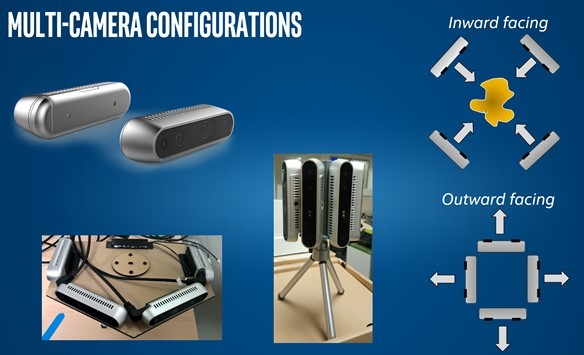
\includegraphics[width=\textwidth]{Figures/Pictures/multicam.jpg}
    \caption{Multi-camera configuration examples. Source: Intel}
    \label{f6.1}
\end{figure}
As we have seen from the previous images we are only working on the face region instead of full head region (including ears). One of the reasons we opted to do so is that one single camera view is not able to capture some parts of the face that are occluded. However, if multiple camera angles will be used this problem will no longer persist and it would be possible to work with a full face model instead of  the reduced model of only the face region. This would also improve the pose estimation process and will most likely produce more accurate shape reconstructions. Thus, we think that it is worthwhile to investigate a multiple camera setup (Figure \ref{f6.1}) and obtain a more accurate and well-structured mesh from a point cloud. The Intel RealSense SDK does provide support for multi-camera setup out of the box\cite{multicam}. Especially useful would be, the inward facing camera configuration from Figure \ref{f6.1}. It will capture the target object from four (or more) different angles and will likely produce full $360^{\circ}$ scan.\bigskip

Additionally, tweaking camera parameters and performing post-processing steps as per \cite{bestcal} could also improve the quality of the target mesh constructed from a point cloud. As we have mentioned in Section \ref{ch3}, there are a lot of configuration parameters available which we did not investigate in detail due to time limitations. Denoising the depth data is one of the obvious optimization steps that would be beneficial for the fitting pipeline\cite{icpram19}. As discussed previously, a point cloud that we obtain from the camera by default is very noisy and lacks the important details and facial characteristics. The higher quality point cloud would most likely produce final reconstructions that are capturing more details of the target face. 

\section{Better Landmark Filtering}
The main reason for our method being very sensitive to the yaw rotation angle is due to Dlib landmarks not being filtered according to the pose. One possible fix of this issue would be to control the Dlib face box during the landmark detection procedure and by doing so only take into account landmark points that are actually visible. Recall, Dlib estimates a location of the landmarks that are not visible in the image and returns a full set of landmarks that are then being de-projected to obtain 3D landmark points. \bigskip

Another work-around would be to assign a higher uncertainty to the landmarks that are being estimated. In our implementation, we have used higher landmark uncertainty for chin landmarks than for the rest of the landmarks. However, we have no way of dynamically detecting the pose variation in the image to ignore altogether or assign higher uncertainty to a subset of landmarks that latter cause problems for the fitting pipeline. We think this is a very important feature update for the entire module since both shape fitting and color fitting module crucially depend on those landmarks. \bigskip

An alternative way to deal with this issue would be to implement a native landmark detection method instead of relying on 3rd party pixel landmark detection method and then de-projection which introduces an additional error. 

\section{Multi-Resolution Fitting}
Unfortunately, due to time constraints, we were not able to deeply research the color fitting module and its speed up capabilities. Because of this, the web service integration was only possible for our shape fitting module. Therefore, we state this challenge as a future work, one possible solution of which could be a multi-resolution fitting. As the name suggests, the basic idea is to perform the color fitting in multiple stages, starting from a low-resolution image and model, and gradually increase the resolution and the complexity of the problem \cite{10.1007/3-540-47967-8_46, surrey809478, visapp16}. \bigskip